\chapter{Diagramy}

\begin{figure}[h]
\begin{center}
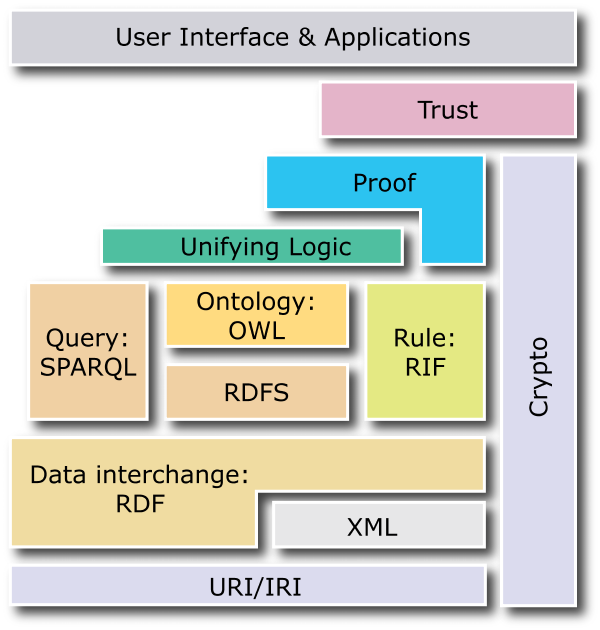
\includegraphics[width=11cm]{figures/SemWebStack}
\caption{Architektura Sémantického webu (navrhl vynálezce WWW Tim Berners-Lee \cite{semWebStack}). (Zdroj \cite{semWeb})}
\label{diagram:SemWebArch}
\end{center}
\end{figure}

\begin{figure}[h]
\begin{center}
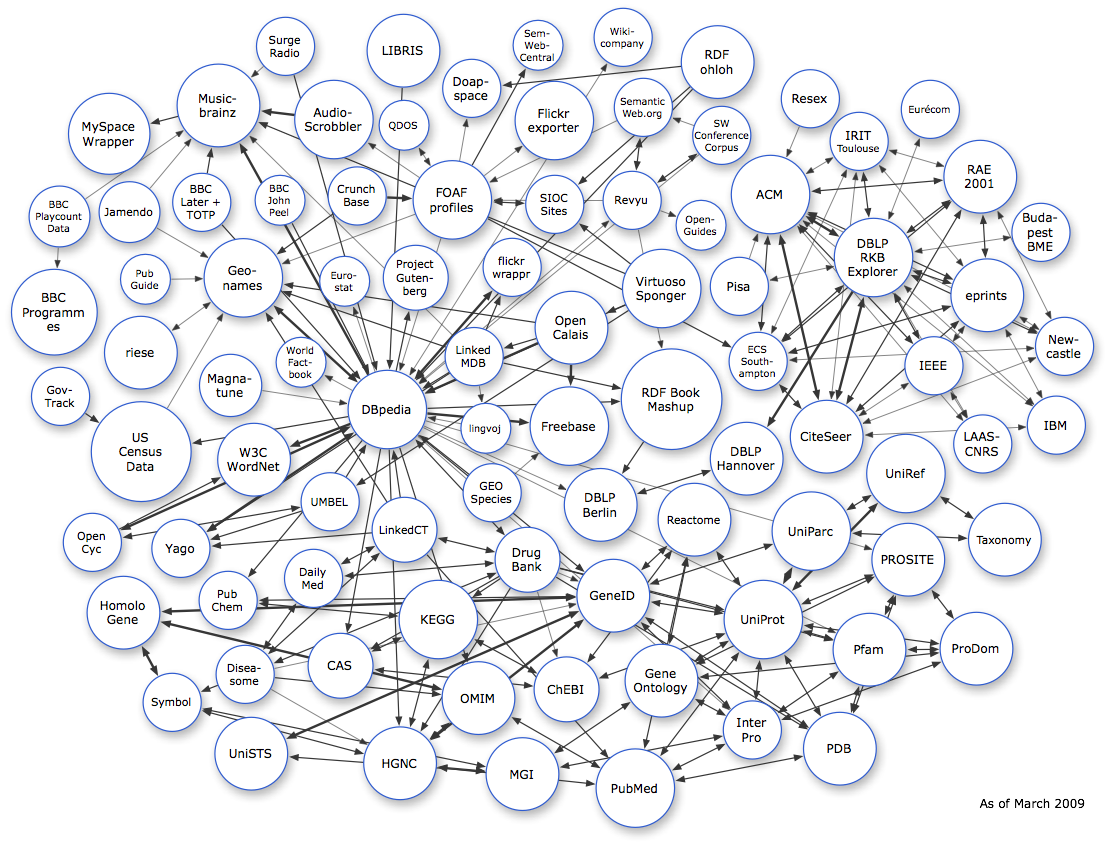
\includegraphics[width=17cm]{figures/linkeddata}
\caption{Graf ontologií (cloud diagram) projektu Linked Data. (Zdroj \cite{linkedData})}
\label{img:linkeddata}
\end{center}
\end{figure}

\begin{figure}[h]
\begin{center}
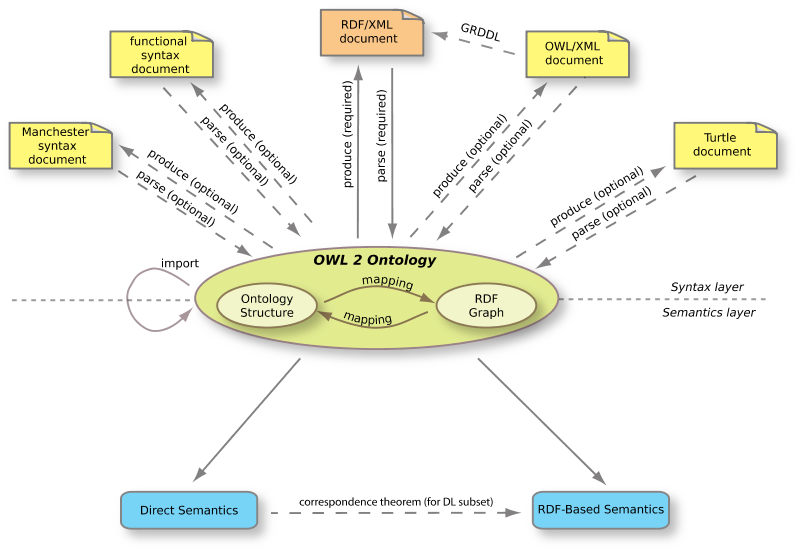
\includegraphics[width=15cm]{figures/OWL2-structure}
\caption{Struktura OWL 2. (Zdroj \cite{owl2})}
\label{img:owl2}
\end{center}
\end{figure}

\begin{figure}[h]
\begin{center}
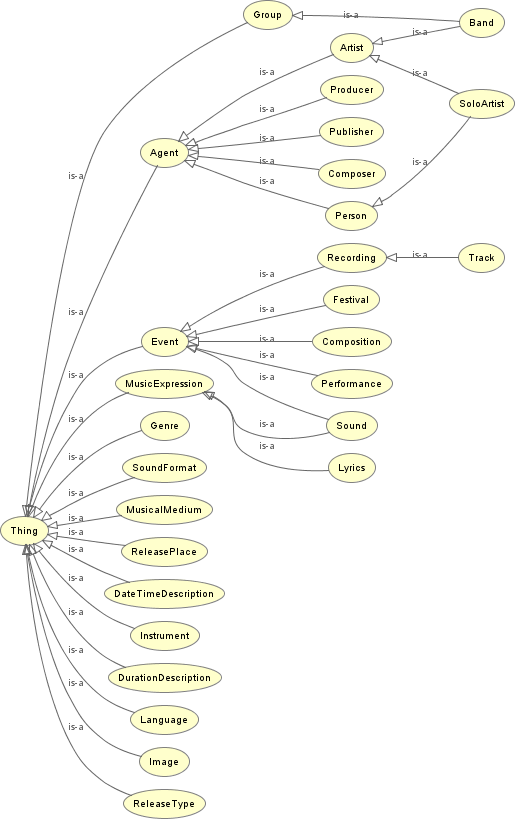
\includegraphics[width=13cm]{figures/mpo_without_genres_instruments}
\caption{Výsledná podoba navržené ontologie (bez hudebních nástrojů a žánrů).}
\label{img:ontoFinal}
\end{center}
\end{figure}

\begin{figure}[h]
\begin{center}
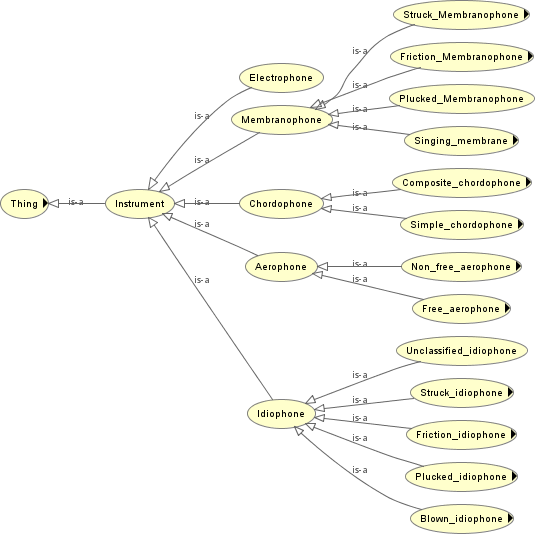
\includegraphics[width=13cm]{figures/mpo_instruments}
\caption{Část struktury tříd hudebních nástrojů podle hudební klasifikace Hornbostel-Sachs.}
\label{img:ontoFinalInstruments}
\end{center}
\end{figure}

\begin{figure}[h]
\begin{center}
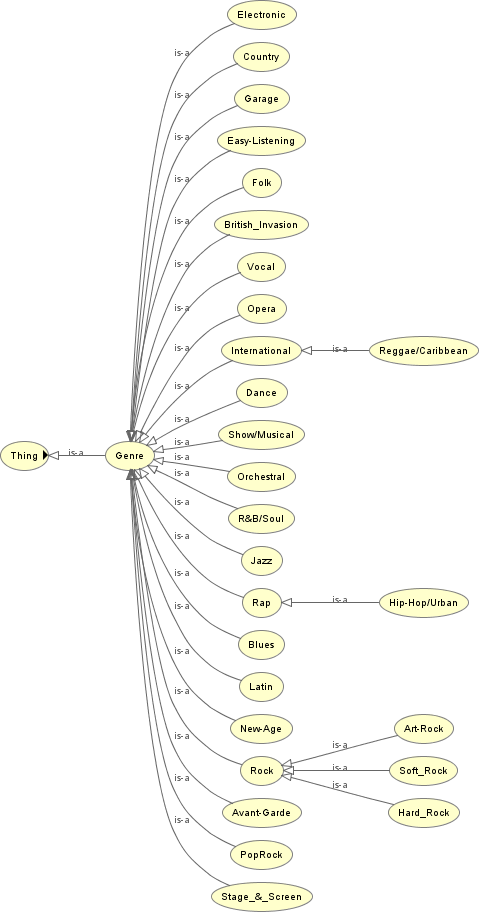
\includegraphics[width=13cm]{figures/mpo_genres}
\caption{Struktura tříd hudebních žánrů.}
\label{img:ontoFinalGenres}
\end{center}
\end{figure}